\section{Einleitung}

''Ärzte und Zahnärzte haben den Anspruch in Ihren Praxen ein Rufsystem einzusetzen.
Dieses Rufsystem ermöglicht, dass der behandelnde Arzt über einen Knopfdruck Hilfe anfordern oder Behandlungsmaterial bestellen kann.''\cite{aufgabenstellung}
Mit diesem Projekt wurde ein cloudbasiertes Praxisrufsystem konzipiert und umgesetzt.
Dieses ermöglicht es Praxismitarbeitenden über Benachrichtigungen und Sprachverbindungen zu kommunizieren.
Dazu wurde eine native iOS Applikation entwickelt, welche als Bedienoberfläche für das System dient.
Folgende Abbildungen zeigen die Startseite der Applikation (Abbildung 1.1) sowie die Ansicht während eines aktiven Gruppenanrufs (Abbildung 1.2).

\begin{figure}[h]
    \centering
    \begin{minipage}[b]{0.4\textwidth}
        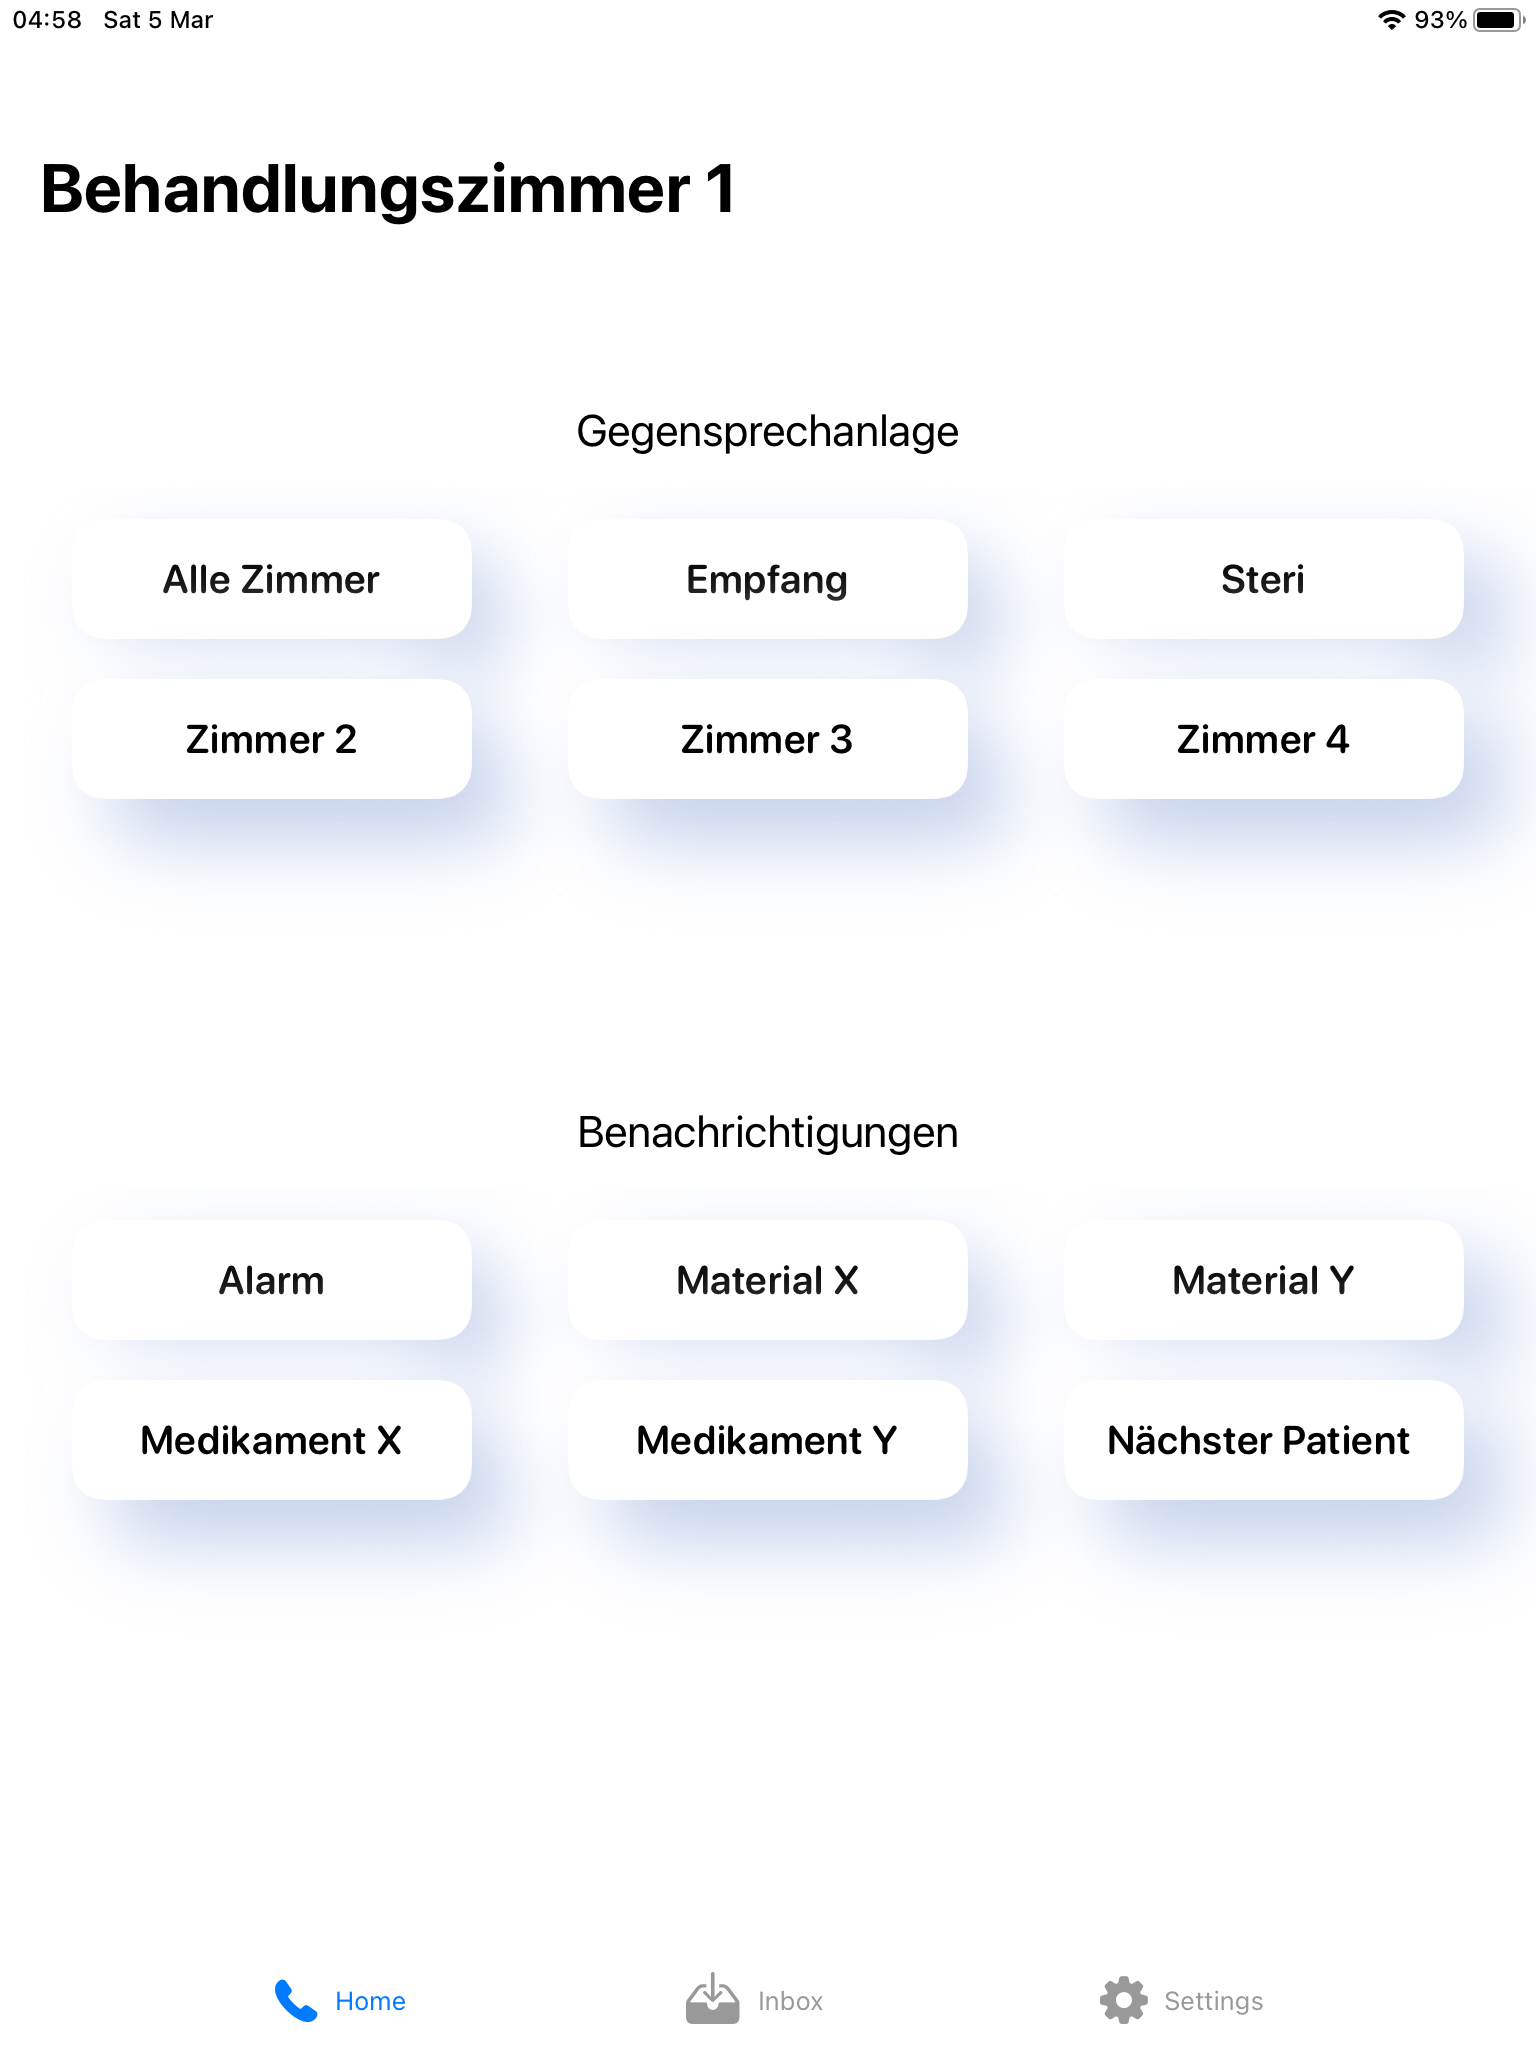
\includegraphics[width=\textwidth]{graphics/screenshots/app/home}
        \caption{Praxisruf Startseite}
    \end{minipage}
    \hfill
    \begin{minipage}[b]{0.4\textwidth}
        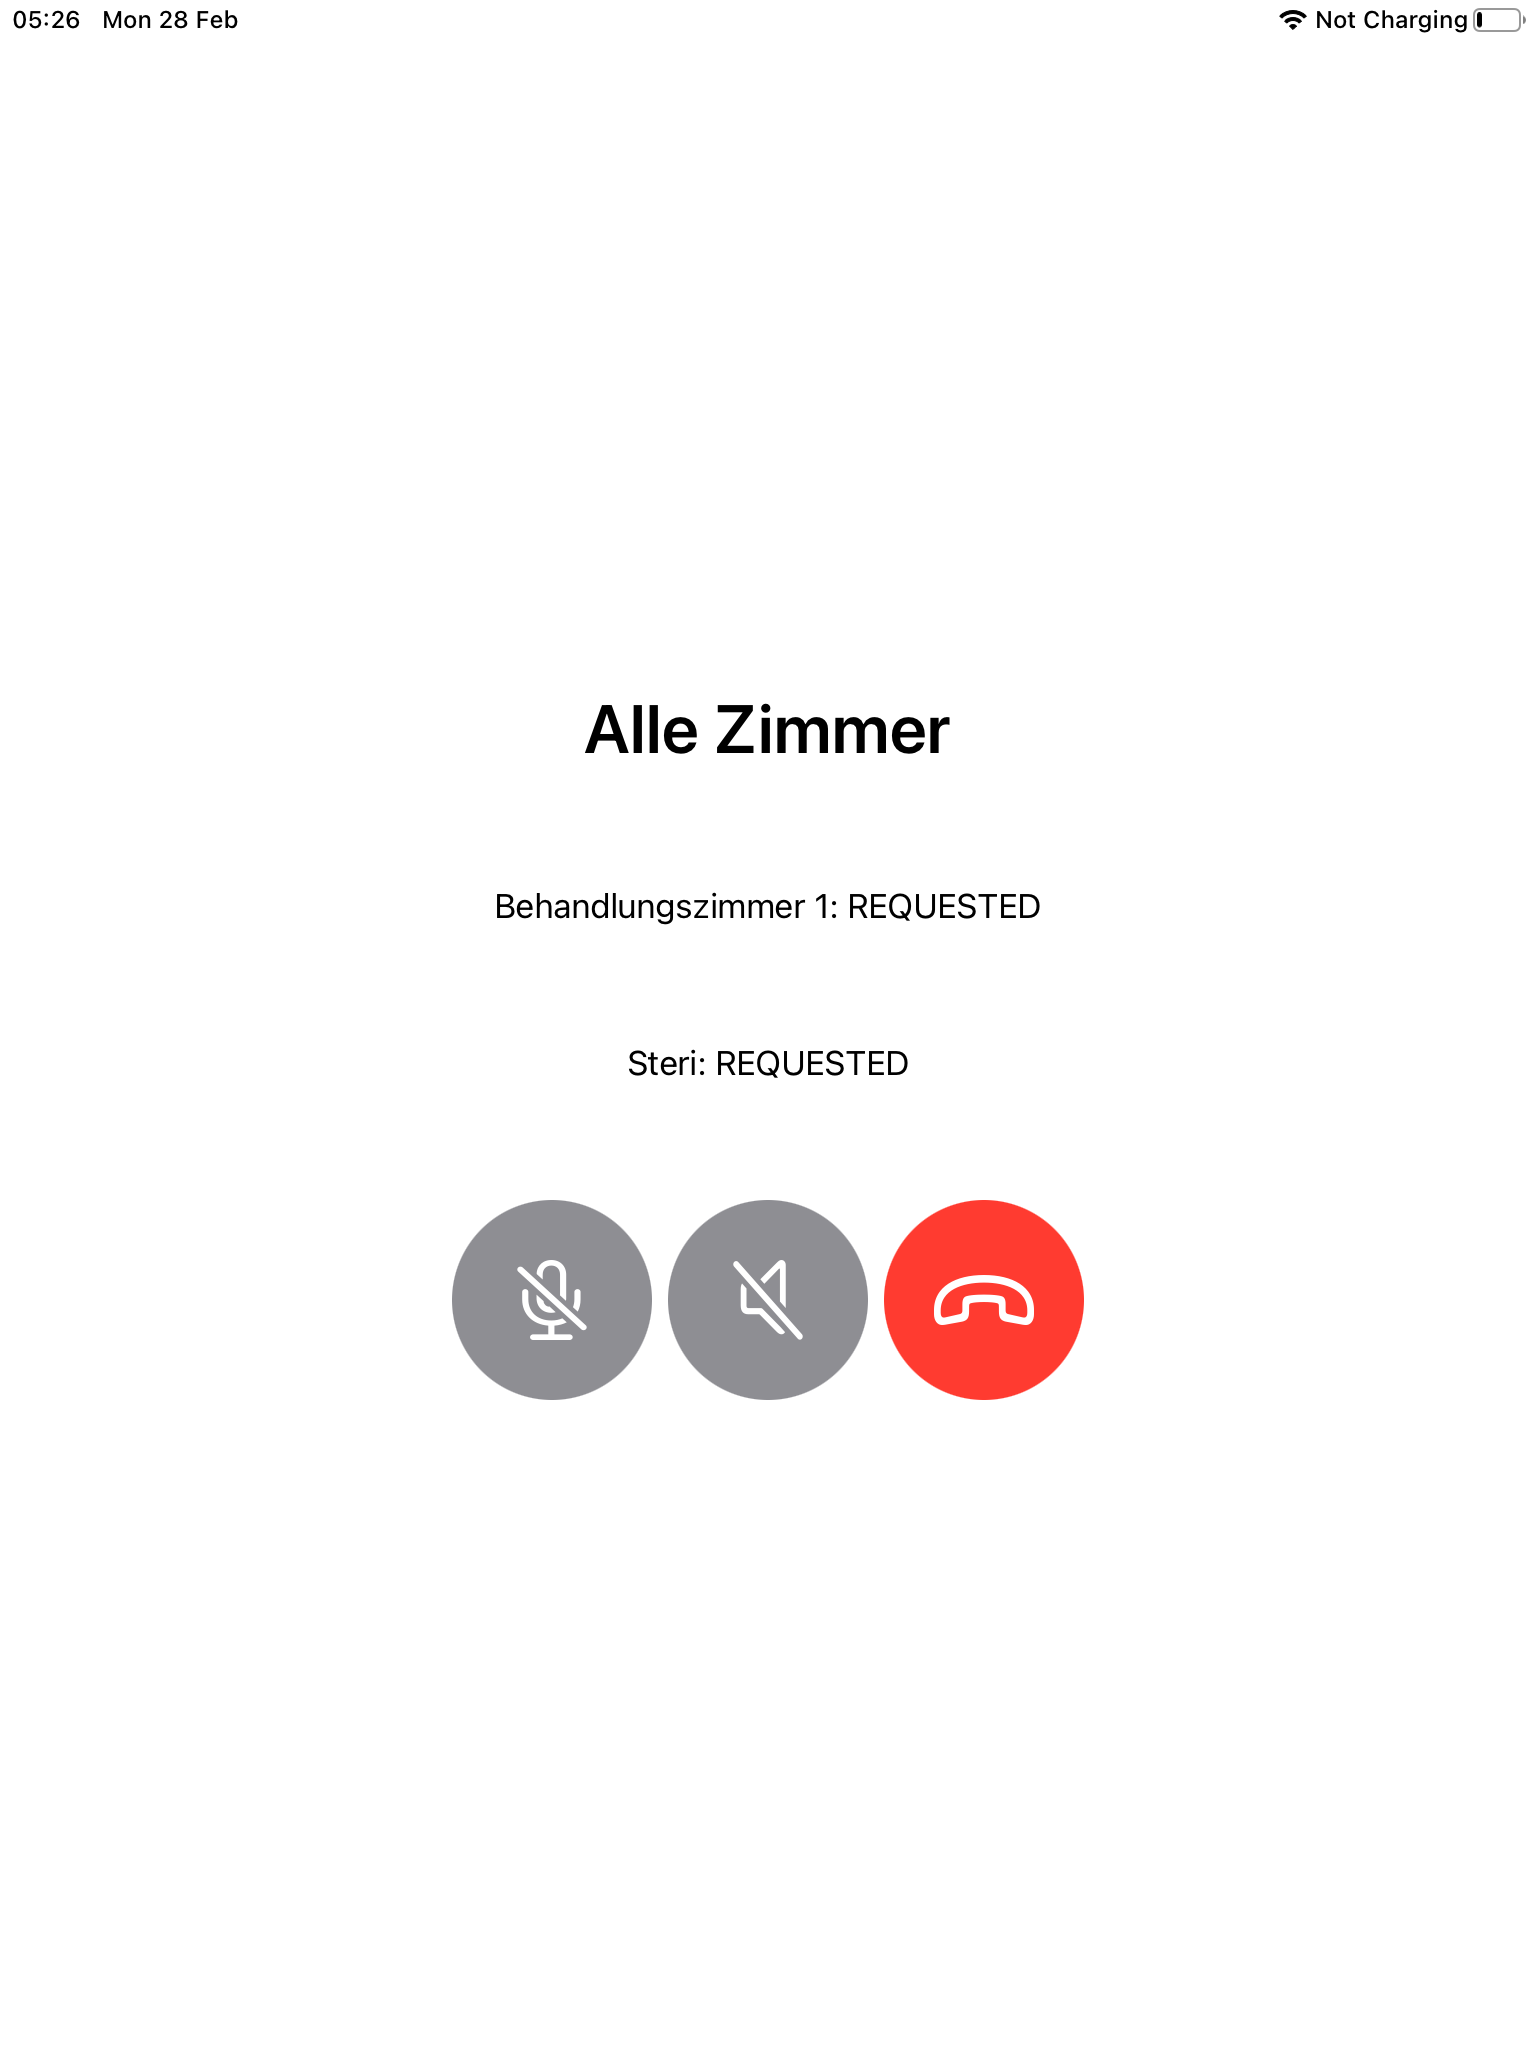
\includegraphics[width=\textwidth]{graphics/screenshots/app/call}
        \caption{Aktiver Anruf}
    \end{minipage}
    \label{fig:MobileClient-ScreensIntroduction}
\end{figure}

Benachrichtigungen und Sprachverbindungen können durch Buttons auf der Startseite der Applikation verwendet werden.
Empfangene Benachrichtigungen werden als Push-Benachrichtigung angezeigt und in einer Inbox gesammelt.
Der Inhalt von empfangenen Benachrichtigungen kann zudem automatisch vorgelesen werden.
Sprachverbindungen können zwischen zwei oder mehr Teilnehmern aufgebaut werden.
Das System unterstützt sowohl private Gespräche als 1:1 Verbindungen wie auch Gruppenunterhaltungen als 1:N Verbindungen.
Welche Buttons und damit welche Benachrichtigungen und Sprachverbindungen zur Verfügung stehen, wird durch Praxisadministratoren konfiguriert.
Die Konfiguration von Buttons für Sprachverbindungen beinhaltet, welche Empfänger für die Verbindung relevant sind.
Die Konfiguration von Buttons für Benachrichtigungen definiert den Inhalt der Benachrichtigung und  welche Empfänger diese erhalten.
Für die Verwaltung dieser Konfiguration kann durch eine Weboberfläche vorgenommen werden.
Abbildung 1.3 zeigt die Übersicht verfügbarer Benachrichtigung in dieser Weboberfläche.

\begin{figure}[h]
    \centering
    \begin{minipage}[b]{1\textwidth}
        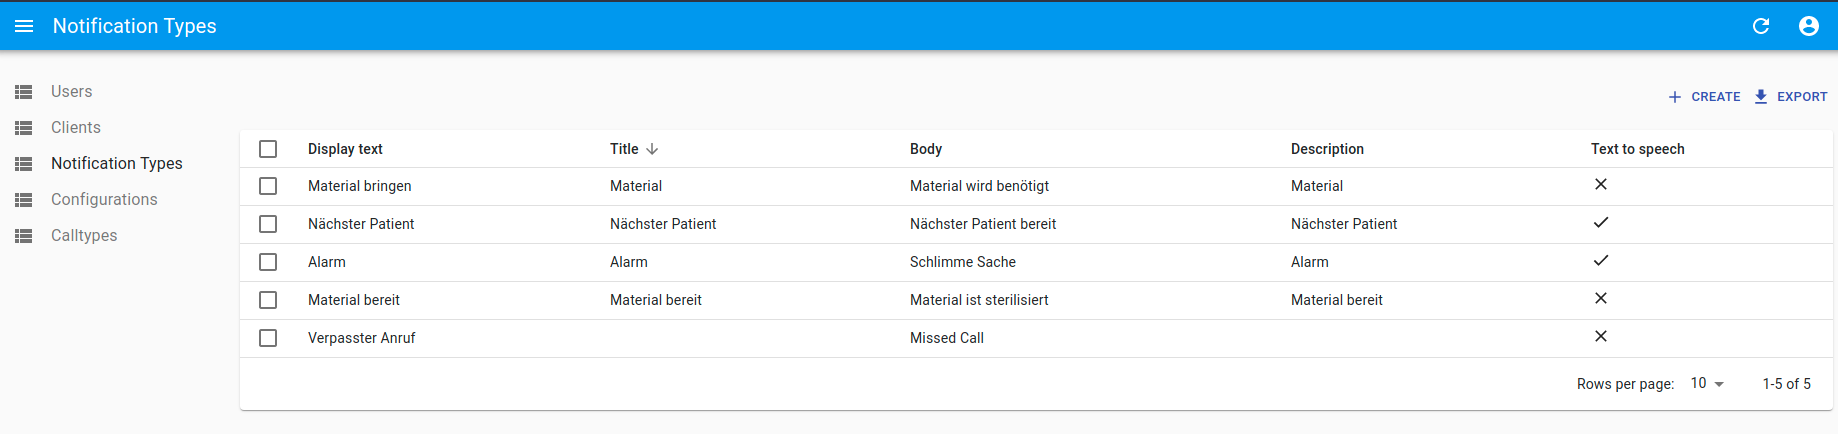
\includegraphics[width=\textwidth]{graphics/screenshots/admin_ui_notification_types}
        \caption{Praxisruf Startseite}
    \end{minipage}
    \label{fig:AdminUI-Introduction}
\end{figure}

Dieses Projekt ist das direkte Nachfolgeprojekt der Projektarbeit ''IP5 Cloudbasiertes Praxisrufsystem''.
Dementsprechend baut die umgesetzte Lösung direkt auf das im Vorgängerprojekt entwickelte System auf.
Das zuvor umgesetzte System unterstützte bereits das Versenden und Empfangen von Benachrichtigungen.
Die Synthese von Sprachdaten und der Aufbau von Sprachverbindungen war damit allerdings noch nicht möglicht.
Mit diesem Projekt wurde das System erweitert um Benachrichtigungen als Sprachdaten synthetisieren und Sprachverbindungen aufbauen zu können.
Weiter wurde die bestehende mobile Applikation von Grund auf neu als native iOS Applikation entwickelt.

Wie in der Aufgabenstellung beschrieben, hat eine Marktanalyse im Vorfeld dieses Projektes gezeigt, dass bestehende kommerzielle Praxisrufsysteme veraltete Technologien einsetzten.
Diese Systeme sind aufwändig zu installieren.
Sie können weiter nicht einfach in ein TCP/IP-Netzwerk eingebunden und über externe APIs angesteuert werden.\cite{aufgabenstellung}
Das cloudbasierte Praxisrufsystem welches mit diesem Projekt umgesetzt wurde, löst diese Probleme.
Im Zentrum dieser Lösung steht eine Serverkomponente mit dem Namen Cloudservice.
Der Cloudservice dient zur Verwaltung der Systemkonfiguration sowie dem Vermitteln von Benachrichtigungen und Sprachverbindungen zwischen Endgeräten.
Verwaltung von Systemkonfiguration und Versenden von Benachrichtigungen wird durch eine Http REST Schnittstelle ermöglicht.
Für den Aufbau von Sprachverbindungen kann der Cloudservice Signalmeldungen über Websocketverbindungen austauschen.
Dies ermöglicht es unter Verwendung dieser Protokolle beliebige Endgeräte an den Cloudservice anzubinden.

Als Endgerät für das umgesetzte System dienen heute iOS Tablets.
Im Rahmen des Vorgängerprojekts wurde bereits eine mobile Applikation umgesetzt, welche das Versenden und Empfangen von Benachrichtigungen unterstützt.
Im Fazit des Vorgängerprojekts wurde festgehalten, dass diese Applikation idealerweise neu als native Applikation entiwckelt werden sollte.
Dadurch könne effizienter Betrieb, Wartung sowie Hardware- und Betriebssystemkomaptibilität langfristig gewährleistet werden.\cite{ip5}
Im Rahmen dieses Projektes wurde der Mobile Client deshalb von Grund auf neu als native iOS Applikation entwickelt.
Die umgesetzte Applikation unterstützt dabei den gesamten Funktionsumfang des Vorgängers sowie die neuen Funktionen Sprachsynthese und Gegensprechanlage.

Im nachfolgenden Hauptteil werden die erarbeiteten Konzepte und Resultate vorgestellt.
Zuerst werden Vorgehensweise, Projektplan und die Organisation für das Projekt.
Anschliessend werden die Anforderungen vorgestellt, welche für Praxisruf umgesetzt werden.
Es wird darauf beschrieben, welche Technologien für die Umsetzung verwendet wurden und begründet, wieso diese Technologien gewählt wurden.
Das Kapitel Konzept beschreibt das detaillierte technische Konzept für Funktionsweise und Architektur von Praxisruf.
Darauf wird das umgesetzte System und Herausforderungen während der Umsetzung vorgestellt.
Am Ende der Arbeit stehen ein Fazit und Schlusswort mit Empfehlungen für das weitere Vorgehen.

\clearpage
